\subsection*{Question 3.1}
In this eksesice we are working on data from 40 hans, representet be 56
points on are 2D plain. One of the hans are shown in figur
\ref{fig:q31hand}, and you can se that the figur loks lige are regular
hand. 

If we take alle the firste x and y, points of the 40 hans. The mean is
calculatet to $[1.0725, 0.4434]$ and the coverianc to $[0.0039, -0.0011;
-0.0011, 0.0005]$, are visualisation of the mean and coveriance, can be
seen in figur \ref{fig:q31onepoint}. wher it can be seen that the gauss
is slitlige tiltet and streats.

If we calculate the mean and coverianc of all the poing in the hans and
plots it. we gets are plot that representent the cance that are given
point of are hand ligs in in the cirkuls in the plot, it can be seen in
figur \ref{fig:q31allpoints}, rekenice that the plot it selv look lik
are hand it self.

\begin{figure}[!htbp]
  \centering
  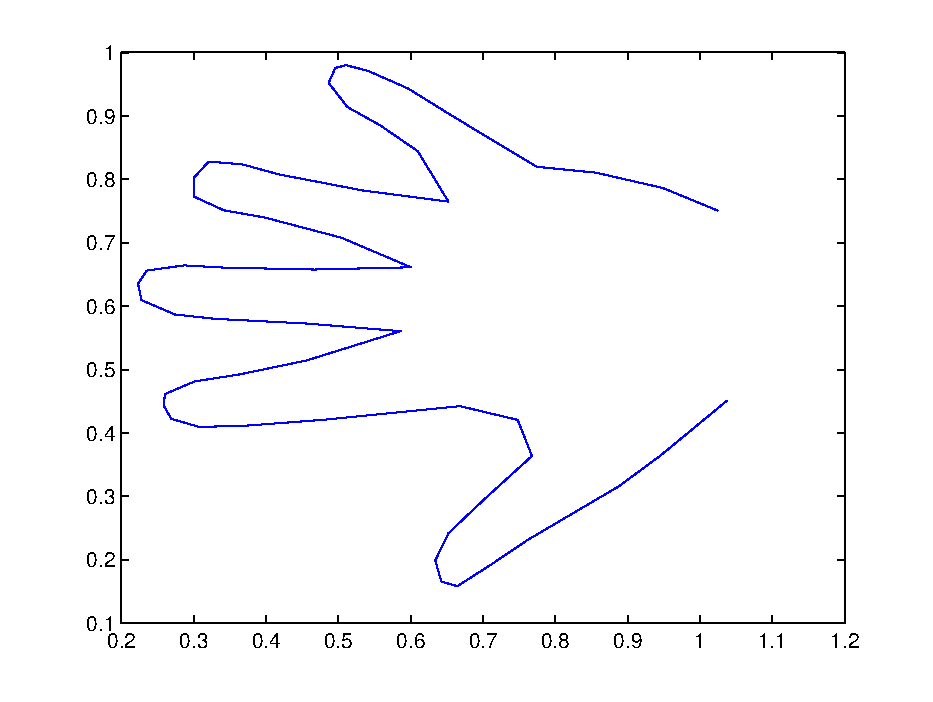
\includegraphics[width=0.85\textwidth]{./images/q31_hand}
  \caption{Shows are plot over the first hand in the data set.}
  \label{fig:q31hand}
\end{figure}

\begin{figure}[!htbp]
  \centering
  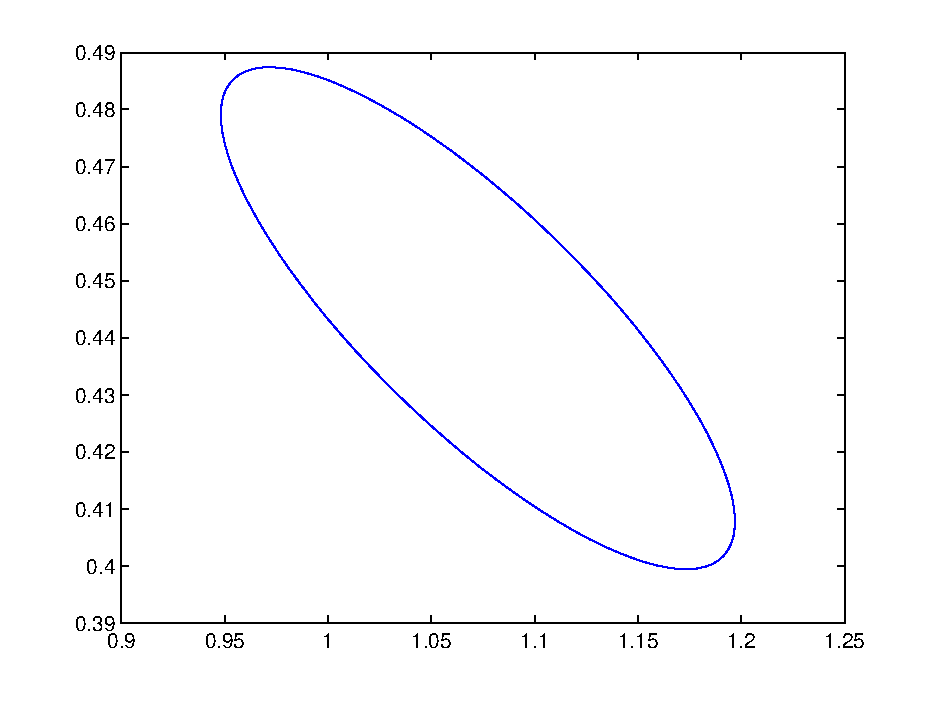
\includegraphics[width=0.85\textwidth]{./images/q31_2}
  \caption{Shows the variation of the first poin af alle the hans.}
  \label{fig:q31onepoint}
\end{figure}

\begin{figure}[!htbp]
  \centering
  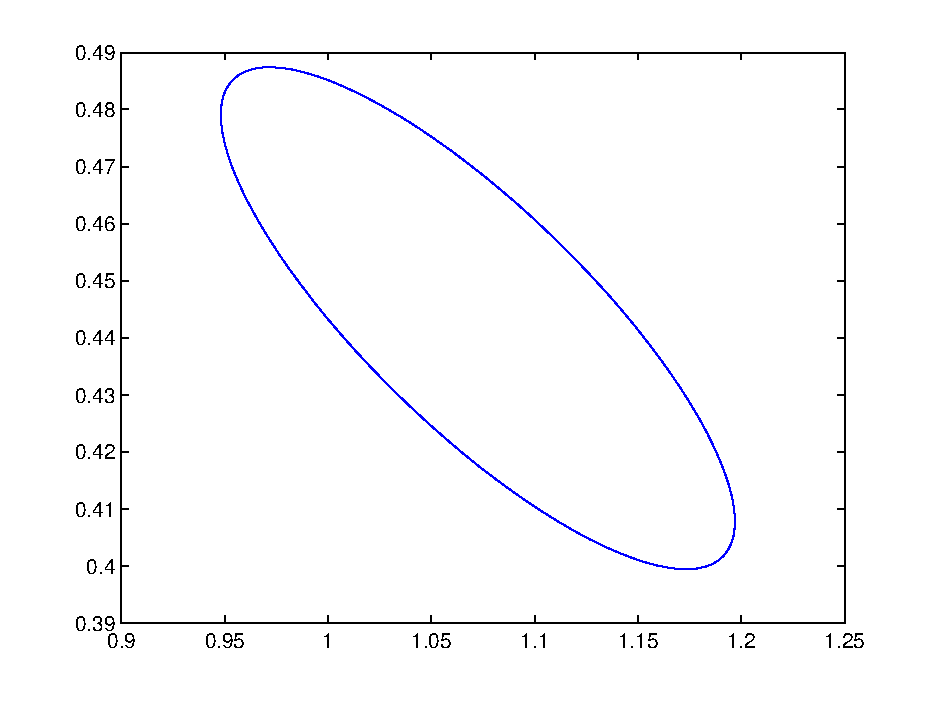
\includegraphics[width=0.85\textwidth]{./images/q31_2}
  \caption{Shows the variation of the first poin af alle the hans.}
  \label{fig:q31allpoints}
\end{figure}

